\section{Non-linear equation system : Quasi-Newton}
Then I had to solve the system of non-linear equation below using Quasi-Newton method.
\begin{equation}
    \begin{cases}
        x_2 sin (\frac{x_1}{2}) - 0.1 = 0 \hspace{1cm}(Z1)\\
        x_1^2 + (\frac{x_2}{4})^4 - 12 = 0 \hspace{1cm}(Z2)
\end{cases}\,
\end{equation}
First, we can plot the surfaces of the two equations, Z1 and Z2.\\
\begin{figure}[H]
    \centering
    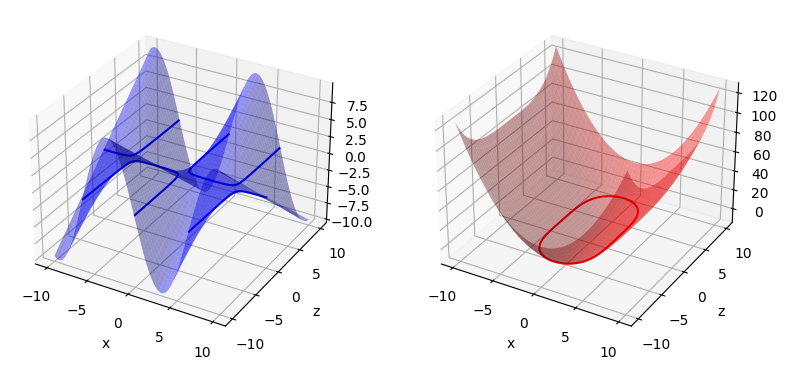
\includegraphics[width=14cm]{images/surfacesrepresntations.png}
    \caption{Z1 (blue) and Z2 (red) surfaces}
    \label{fig:surfacesplots}
\end{figure}
The lines represent the values in which the equation is equal to 0.\\
Then we can plot the intersections of the two surfaces, and even the intersections of the lines, which will give us the solutions graphically.
\begin{figure}[H]
    \centering
    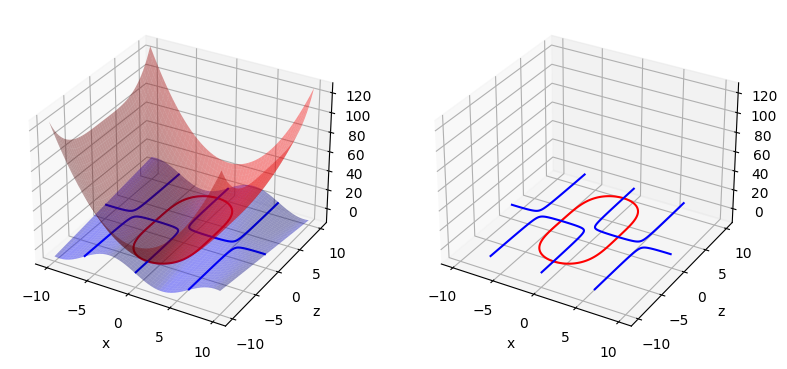
\includegraphics[width=14cm]{images/solutionrepresentations.png}
    \caption{Z1 (blue) and Z2 (red) surfaces intersections}
    \label{fig:solutionsplots}
\end{figure}

To code the Quasi-Newton algorithm, we will need the function and its Jacobian matrix (obtained with approximations of the partial derivates of the function).\\
\begin{lstlisting}[language=Python, style=jupycolors]
def fnleq(x):
    return np.array( [x[1]*np.sin(0.5*x[0])-0.1, 
                      x[0]**2+(0.25*x[1])**4-12])

def quasidfi(f, i, x, j):
    h = 1e-6
    xh = []
    for k in range(len(x)):
        if k == i:
            xh.append(x[k] + h)
        else:
            xh.append(x[k])
    y = f(x)[j]
    yh = f(xh)[j]
    r = (yh - y) / h
    #print("r :", r)
    return r
        

def Jf(fct, x, nbeq):
    multigrad = []
    for f in range(nbeq):
        grad = []
        for i in range(len(x)):
            grad.append(quasidfi(fct, i, x, f))
        multigrad.append(grad)
    return np.array(multigrad)
\end{lstlisting}
The Quasi-Newton algorithm takes as argument an initial point (with two coordinates in our case), and do several iterations to make this point converge to a root.\\
\begin{lstlisting}[language=Python, style=jupycolors]
def QuasiNewton(f, x, eps):
    maxsteps = 2000
    step = 0
    while (step < maxsteps and np.any(abs(f(x)) > eps)):
        step += 1
        #print("xi : ", x)
        #print("s: ", step, " | Jf : ", Jf(f, x, 2))
        jxtmp = Jf(f, x, 2)
        jxl = jxtmp.tolist()
        if np.abs(jxl[0][0]) < .001 and np.abs(jxl[0][1]) < .001 and np.abs(jxl[1][1]) < .001 and np.abs(jxl[1][0]) < .001 :
            return False, step
        x = np.array(x) - np.linalg.inv(jxtmp)@f(x)
    return x, step
\end{lstlisting}
Finally, to find all the roots we make a whole set of points (in my case I made a grid of 16 points distributed on our surface of interest (-10 to 10 for the two axis))\\
\begin{lstlisting}[language=Python, style=jupycolors]
def createSet(xmin, xmax, ymin, ymax, resolution):
    xy = []
    for yi in range(resolution + 1):
        yivals = []
        yval = ymin + yi * (ymax - ymin) / resolution
        for xi in range(resolution + 1):
            xval = xmin + xi * (xmax - xmin) / resolution
            yivals.append([xval, yval])
        xy.append(yivals)
    return xy

def getAllFromQuasiNewton(f, xy, rooteps):
    sols = []
    totalsteps = 0
    numberofpoints = 0
    # print("Before newton")
    # printcoords(xy)
    for i in range(len(xy)):
        for j in range(len(xy[i])):
            newsol, steps = QuasiNewton(f, xy[i][j], 1e-8)
            totalsteps += steps
            numberofpoints += 1
            if not isinstance(newsol, bool):
                xy[i][j] = newsol.tolist()
                found=False
                for s in sols:
                    if abs(s[0] - newsol[0]) < rooteps and abs(s[1] - newsol[1]) < rooteps:
                        found=True
                if not found:
                    sols.append(newsol.tolist())
                    #print("NEW : ", sols)
    # print("After newton")
    # printcoords(xy)
    print("Average number of steps per point:", totalsteps/numberofpoints)
    return sols
            

def printcoords(xy):
    print("[")
    for y in xy:
        for x in y:
            print(x, end=", ")
        print("")
    print("]")


xy = createSet(-10, 10, -10, 10, 4)
printPoints(xy)
\end{lstlisting}
\begin{figure}[H]
    \centering
    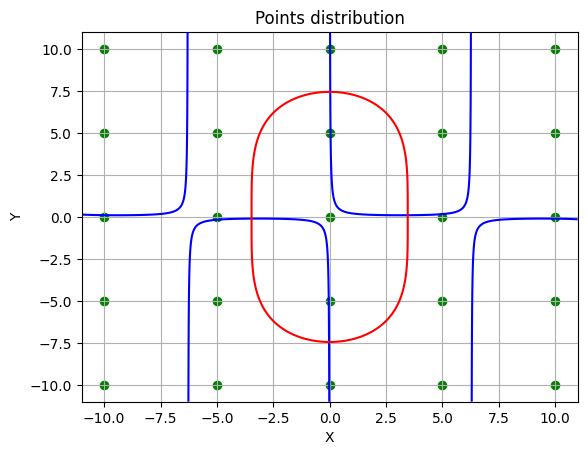
\includegraphics[width=10cm]{images/nldistribution.png}
    \caption{Set of distributed points on which Quasi-Newton will be applied}
    \label{fig:nldistri}
\end{figure}
Then we start Quasi-Newton method on every point and see where they converge.
\begin{lstlisting}[language=Python, style=jupycolors]
v = getAllFromQuasiNewton(fnleq, xy, 0.1)
print("Solutions of the non-linear equation are : ")
print(v)
printSolutions(v)
\end{lstlisting}
So finally we obtain the approximated coordinates of the 4 solutions:\\
\begin{resultbox}
    Average number of steps per point: 30.64\\
    Solutions of the non-linear equation are : \\
    $[[-0.026865460174149012, -7.4447269258435576],$\\
    $[-3.4641015557326065, -0.10131438702733254],$\\
    $[3.4641015559745827, 0.10131438728799054],$\\
    $[0.026865460174157533, 7.444726925845088]]$
\end{resultbox}
\begin{figure}[H]
    \centering
    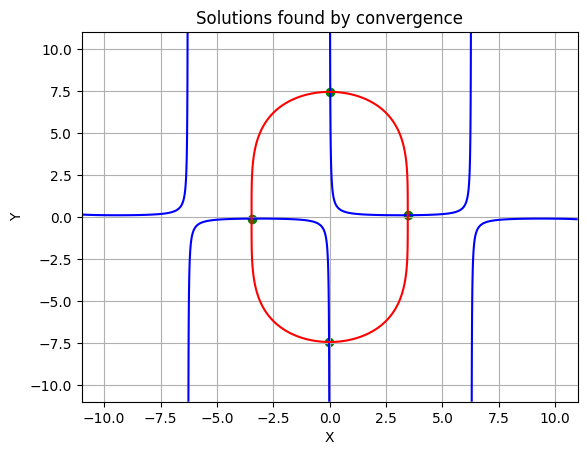
\includegraphics[width=10cm]{images/nlconvergence.png}
    \caption{Points convergence after Quasi-Newton method}
    \label{fig:nlconv}
\end{figure}

To verify the results, I used the website \url{https://www.wolframalpha.com/}.
\begin{figure}[H]
    \centering
    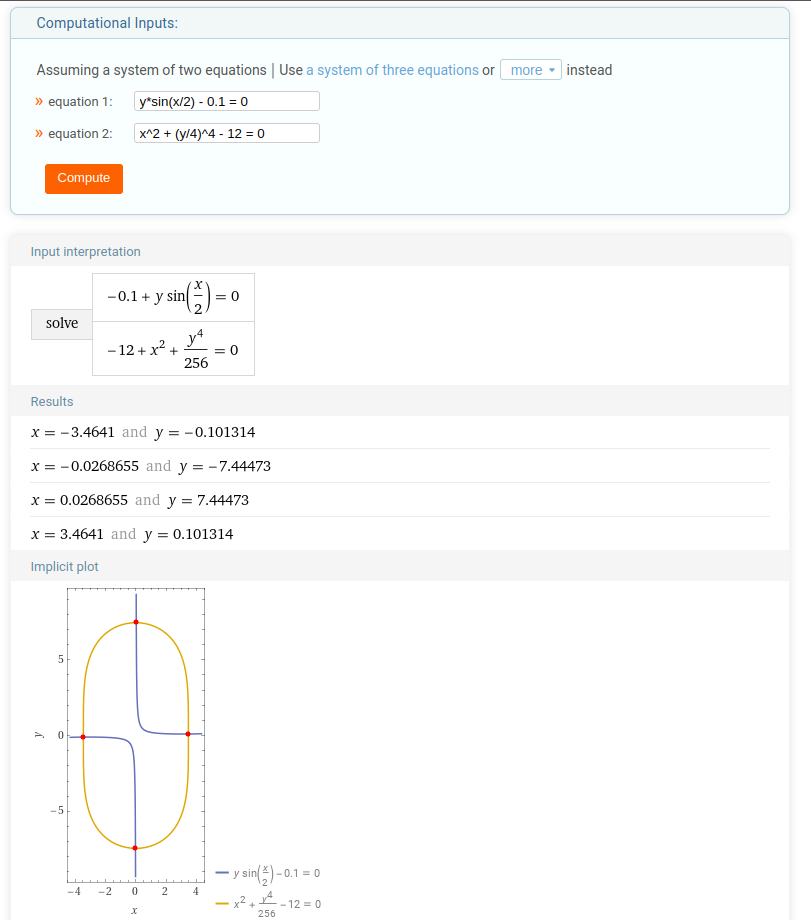
\includegraphics[width=10cm]{images/verifNonLinear.png}
    \caption{WolframAlpha results}
    \label{fig:wolframNonLinear}
\end{figure}